% ****** Start of file aipsamp.tex ******
%
%   This file is part of the AIP files in the AIP distribution for REVTeX 4.
%   Version 4.1 of REVTeX, October 2009
%
%   Copyright (c) 2009 American Institute of Physics.
%
%   See the AIP README file for restrictions and more information.
%
% TeX'ing this file requires that you have AMS-LaTeX 2.0 installed
% as well as the rest of the prerequisites for REVTeX 4.1
%
% It also requires running BibTeX. The commands are as follows:
%
%  1)  latex  aipsamp
%  2)  bibtex aipsamp
%  3)  latex  aipsamp
%  4)  latex  aipsamp
%
% Use this file as a source of example code for your aip document.
% Use the file aiptemplate.tex as a template for your document.
\documentclass[%
 aip,12pt
% jmp,
% bmf,
% sd,
% rsi,
 amsmath,amssymb,
%preprint,%
 reprint,%
%author-year,%
%author-numerical,%
% Conference Proceedings
]{revtex4-1}
\citestyle{ieeetr}

\usepackage{dcolumn}% Align table columns on decimal point
\usepackage{bm}% bold math

%\usepackage[mathlines]{lineno}% Enable numbering of text and display math
%\linenumbers\relax % Commence numbering lines
\usepackage{tikz}
\usepackage[utf8]{inputenc}
\usepackage[T1]{fontenc}
\usepackage{mathptmx}
\usepackage{etoolbox}

\usepackage{tikz-network}
%% Apr 2021: AIP requests that the corresponding
%% email to be moved after the affiliations
\makeatletter
\def\@email#1#2{%
 \endgroup
 \patchcmd{\titleblock@produce}
  {\frontmatter@RRAPformat}
  {\frontmatter@RRAPformat{\produce@RRAP{*#1\href{mailto:#2}{#2}}}\frontmatter@RRAPformat}
  {}{}
}%
\makeatother
\begin{document}

%\preprint{AIP/123-QED}

\title[Fast and Accurate Randomized Algorithms For the Eigenvalue Problem in the Tensor Train Format]{Fast and Accurate Randomized Algorithms For the Eigenvalue Problem in the Tensor Train Format
}
% Force line breaks with \\
\author{Christian Camano}
\affiliation{San Francisco State University}
\author{Roel Van Beeumen}%
\affiliation{Lawrence Berkeley National Laboratory}
\date{\today}% It is always \today, today,
             %  but any date may be explicitly specified

\begin{abstract}
\textbf{Abstract.}.
We present an overview of tensor sketching for the eigenvalue problem. Our discussion evaluates the practicality of a number of randomized sketching techniques and their analogs in the tensor train format. Special attention is given to the sketched Rayleigh-Ritz method for the computation of eigenpairs and the generalized Nyström technique for random sketching. Figures demonstrating the structure of the modified tensor networks are given.
\end{abstract}

\maketitle


\subsubsection{\label{sec:level3}Introduction}
One of the greatest challenges in contemporary numerical linear algebra research is finding efficient ways to represent high dimensional data. Due to restrictions in available physical memory and the exponential nature of many scientific problems there has been a push over the last decade to develop fast alternative solutions to the deterministic algorithms that preceded the current era of applied mathematics. Random matrix theory has proven to be an effective response to this problem and leverages the concept of dimensionality reduction to create near approximations to desired information by solving local problems in a lower dimensional vector space and projecting back into the problem space once a local answer has been computed.
\\
Additionaly, The Tensor Train (TT) format [1] can also aid in this domain by enabling the efficient expression of large matrices. Originally developed in the domain of physics TT has been used for some time under another name Matrix Product State(MPS).
\\
This paper aims to explore some of the possible ways the that TT can be used in conjunction with randomized algorithms to create a new class of fast and accurate eigensolvers that avoids the current precedent of reformatting the problem as a sum of small optimizations. Current iterative solvers in the TT format have a tendency to rely on sweeping algorithms that ocassionally stagnate in local minima during optimization. We are currently investigating the theoretical side of this area of research with results and numerical simulations pending.
\subsubsection{\label{sec:level3}The Tensor Train format}
In this section we describe an introduction to the \emph{Tensor Train} (TT) format. The major idea of the TT format is to seperate the modes of a tensor into \emph{d} order-2 or order-3 tensors. The result is a tensor network that when contracted over the bond indicies can be used to reform the original input.
 \\\\
 \textbf{Definition 1} (Tensor Train Format)
 Let $X \in \mathbb{R}^{n_1\times...\times n_d}$ be a tensor of order $d$. The decomposition of $X$
\begin{eqnarray}
   X=X^{(1)}\circ X^{(2)}\circ...\circ X^{(d-1)}\circ X^{(d)}
\label{eq:one}
\end{eqnarray}
into component tensors  $X^{(i)}\in \mathbb{R}^{r_{i-1}\times n_i \times r_i}$ for i=$1,...,d$ is called a tensor train (TT) representation of $X$. It is assumed that $r_0=r_N=1$. \\
\\
An example resultant tensor network of this format is shown for an order-5  tensor
$X=X^{(1)}\circ X^{(2)}\circ X^{(3)}\circ X^{(4)}\circ X^{(5)}}$ in the following diagram

\begin{center}
  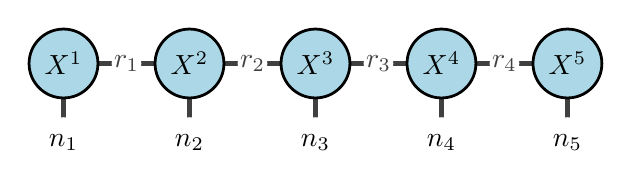
\begin{tikzpicture}
%First node
  \Vertex[label=$X^{1}$,fontsize=\normalsize,size=.875,x=0,y=0]{A}
  \Vertex[style={color=white},label=$n_1$,fontsize=\normalsize,x=0,y=-1]{Aa}
  \Edge[Math](A)(Aa)
% Second node
  \Vertex[label=$X^{2}$,fontsize=\normalsize,size=.875,x=1.6]{B}
  \Vertex[style={color=white},label=$n_{2}$,fontsize=\normalsize,x=1.6,y=-1]{Bb}
  \Edge[Math](B)(Bb)
  %Fake node
  %\Vertex[style={color=white},label=$⎯ ⎯ ⎯$,fontcolor=black,fontsize=\normalsize,x=1.2,y=]{X}
% bond
  \Edge[Math,label={r_1},fontsize=\normalsize](A)(B)
  %\Edge[Math,style={dashed},label=r_1,fontsize=\normalsize](X)(B)

%Third node
  \Vertex[label=$X^{3}$,fontsize=\normalsize,size=.875,x=3.2,y=0]{C}
  \Vertex[style={color=white},label=$n_3$,fontsize=\normalsize,x=3.2,y=-1]{Cc}
  \Edge[Math](C)(Cc)
% bond
    \Edge[Math,label=r_2,fontsize=\normalsize](B)(C)
%fourth node
  \Vertex[label=$X^{4}$,fontsize=\normalsize,size=.875,x=4.8,y=0]{D}
  \Vertex[style={color=white},label=$n_{4}$,fontsize=\normalsize,x=4.8,y=-1]{Dd}
  \Edge[Math](D)(Dd)
% bond
    \Edge[Math,label=r_3,fontsize=\normalsize](C)(D)
%Fifth node
  \Vertex[label=$X^{5}$,fontsize=\normalsize,size=.875,x=6.4,y=0]{E}
  \Vertex[style={color=white},label=$n_5$,fontsize=\normalsize,x=6.4,y=-1]{Ee}
  \Edge[Math](E)(Ee)
% bond
    \Edge[Math,label=r_4,fontsize=\normalsize](D)(E)
  \end{tikzpicture}\\
  Figure 1: Example of tensor train vector of order-5
\end{center}


This decomposition is traditionally formed by using succesive singular value decompostitions in which at each step a (matrix) SVD is preformed to detach one open mode from the TT. For a complete description on the formation of a tensor train from a starting tensor see the work of Oseldets [1]
The space complexity for a TT format is $\mathcal{O}(nNr^2)$ where $r=max(r_n)$, $N$ is the order and  $n=max(n_k)$.\\
\subsubsection{\label{sec:level3} The eigenvalue problem expressed in TT }

A well known eigenvalue algorithm that utilizes the tensor train format is the  density-matrix renormalization group (DMRG) which computes the loweset wavefunction of a Hamiltonian. This information can be encoded within the extreme eigenvalues of the matrix as well and is often expressed using this perspective. \\
DMRG was first adapted for the TT format by Dolgolov and Oseletes [5] using a modified version of the alternating least squares method. The algorithm preforms a sweeping motion over the Tensor Train solving small local eigenproblems until the Tensor Train vectors closely approximate the true eigenvector of the global system.
\\
This algorithm, while very effective,  is still largely dependent on the Locally Optimal Block Preconditioned Conjugate Gradient (LOBPCG) [6] method for the computation of the local solutions, creating a computational bottleneck when local problems themselves are large as well.\\
Alternative algorithms such as sRR theoretically could enable the computation of approximate eigenvectors without the need for an iterative approach that breaks the larger problem down into local systems. Such an algorithm would consist of uniform contraction between TT matrix cores and TT vector cores in the optimization of the Rayliegh quotient problem:

\begin{eqnarray}
  \text{min trace}_X(X^*AX)\quad s.t. X^*X=I
  \label{eq:five}
\end{eqnarray}
 where $X$ is the the eigenvectors of the system expressed in TT vector format. \\
 In DMRG  the notion of a blocked tensor train core is used to allow for the computation of the trace in the local problem. This blocked core is a core of a tensor train in which an additional index $b$ is added to a given core
 \begin{eqnarray}
 \dots X^{(k-1)}\left(i_{k-1}\right) \widehat{X}^{(k)}\left(i_{k}, b\right) X^{(k+1)}\left(i_{k+1}\right) \ldots
\end{eqnarray}
The choice of which mode $k$ expressed in the block format changes as the tensor train is optimized with the selection walking back and forth along the tensor train in a sweeping motion until a tolerance criteria for the eigenvector approximation is met.

\\
Two interface cores are constructed from the remaning tensor train to the left and right of the selected core that was re-expressed in block format as follows:
\begin{equation}
\begin{split}
&X^{<k}\left(\overline{i_{1} i_{2} \ldots i_{k-1}}, \beta_{k-1}\right)=
\\
&\sum_{\alpha_{1} \ldots \alpha_{k-2}} X_{\alpha_{1}}^{(1)}\left(i_{1}\right) X_{\alpha_{1} \alpha_{2}}^{(2)}\left(i_{2}\right) \ldots X_{\alpha_{k-2}, \beta_{k-1}}^{(k-1)}\left(i_{k-1}\right) \\
&X^{>k}\left(\beta_{k}, \overline{i_{k+1} \ldots i_{d-1} i_{d}}\right)=
\\
&\sum_{\alpha_{k+1} \ldots \alpha_{d-1}} X_{\beta_{k}, \alpha_{k+1}}^{(k+1)}\left(i_{k+1}\right) \ldots X_{\alpha_{d-2}, \alpha_{d-1}}^{(\mathrm{d}-1)}\left(i_{d-1}\right) X_{\alpha_{d-1}}^{(\mathrm{d})}\left(i_{d}\right)
  \end{split}
  \end{equation}

Using the interfaces a frame matrix is then defined as

\begin{equation}
  X_{\neq k}=X^{<k} \otimes I_{n_{k}} \otimes\left(X^{>k}\right)^{\top},
\end{equation}

Using these newly formed tensor cores we can now re-express the original eigen problem as a local framed problem.

\begin{equation}
  \text{min trace}_X((X^k)^TX_{\neq k}^TA^kX_{\neq k}X^k)
\end{equation}
Where $A^k$ is the $k^{th}$ core of the TT matrix $A$ and the current site of local optimization\\
\\\\
\begin{center}
  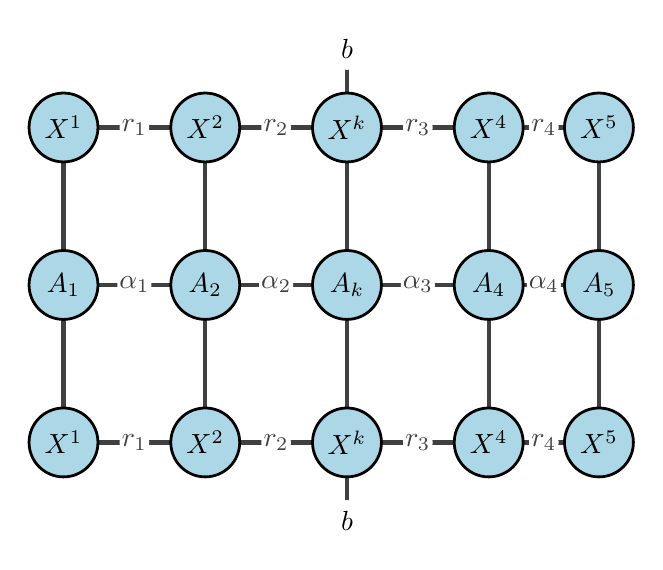
\begin{tikzpicture}
%First node
  \Vertex[label=$X^{1}$,fontsize=\normalsize,size=.875,x=0,y=0]{A}
  \Vertex[,label=$A_1$,fontsize=\normalsize,size=.875,x=0,y=-2]{Aa}
  \Vertex[,label=$X^1$,fontsize=\normalsize,size=.875,x=0,y=-4]{Aaa}
  \Edge[Math](A)(Aa)
  \Edge[Math](Aa)(Aaa)
% Second node
  \Vertex[label=$X^{2}$,fontsize=\normalsize,size=.875,x=1.8]{B}
  \Vertex[,label=$A_2$,fontsize=\normalsize,size=.875,x=1.8,y=-2]{Bb}
  \Vertex[,label=$X^2$,fontsize=\normalsize,size=.875,x=1.8,y=-4]{Bbb}
  \Edge[Math](B)(Bb)
    \Edge[Math](Bb)(Bbb)
% bond
  \Edge[Math,label={r_1},fontsize=\normalsize](A)(B)
  \Edge[Math,label={\alpha_1},fontsize=\normalsize](Aa)(Bb)
  \Edge[Math,label={r_1},fontsize=\normalsize](Aaa)(Bbb)
  %\Edge[Math,style={dashed},label=r_1,fontsize=\normalsize](X)(B)

%Third node
  \Vertex[label=$b$,style={color=white},fontsize=\normalsize,size=.5,x=3.6,y=1]{o}
  \Vertex[label=$X^{k}$,fontsize=\normalsize,size=.875,x=3.6,y=0]{C}
  \Vertex[,label=$A_k$,fontsize=\normalsize,size=.875,x=3.6,y=-2]{Cc}
  \Vertex[,label=$X^k$,fontsize=\normalsize,size=.875,x=3.6,y=-4]{Ccc}
  \Vertex[label=$b$,style={color=white},fontsize=\normalsize,size=.5,x=3.6,y=-5]{p}
 \Edge[Math](o)(C)
  \Edge[Math](C)(Cc)
  \Edge[Math](Cc)(Ccc)
  \Edge[Math](Ccc)(p)
% bond
    \Edge[Math,label=r_2,fontsize=\normalsize](B)(C)
    \Edge[Math,label=\alpha_2,fontsize=\normalsize](Bb)(Cc)
    \Edge[Math,label=r_2,fontsize=\normalsize](Bbb)(Ccc)
%fourth node
  \Vertex[label=$X^{4}$,fontsize=\normalsize,size=.875,x=5.4,y=0]{D}
  \Vertex[,label=$A_4$,fontsize=\normalsize,size=.875,x=5.4,y=-2]{Dd}
  \Vertex[,label=$X^4$,fontsize=\normalsize,size=.875,x=5.4,y=-4]{Ddd}
  \Edge[Math](D)(Dd)
    \Edge[Math](Dd)(Ddd)
% bond
    \Edge[Math,label=r_3,fontsize=\normalsize](C)(D)
    \Edge[Math,label=\alpha_3,fontsize=\normalsize](Cc)(Dd)
    \Edge[Math,label=r_3,fontsize=\normalsize](Ccc)(Ddd)
%Fifth node
  \Vertex[label=$X^{5}$,fontsize=\normalsize,size=.875,x=6.8,y=0]{E}
  \Vertex[,label=$A_5$,fontsize=\normalsize,size=.875,x=6.8,y=-2]{Ee}
  \Vertex[,label=$X^5$,fontsize=\normalsize,size=.875,x=6.8,y=-4]{Eee}
  \Edge[Math,](E)(Ee)
  \Edge[Math](Ee)(Eee)
% bond
    \Edge[Math,label=r_4,fontsize=\normalsize](D)(E)
    \Edge[Math,label=\alpha_4,fontsize=\normalsize](Dd)(Ee)
    \Edge[Math,label=r_4,fontsize=\normalsize](Ddd)(Eee)
  \end{tikzpicture}
    Figure 2: Example construction of minimization of the rayleigh quotient over local eigenproblem.
\end{center}
\begin{center}

\end{center}
While the DMRG approach to this problem appears to be limited by its dependence of LOBPCG it does reveal a practical framing scheme for local problems that can be used when considering randomized techniques.

\subsubsection{\label{sec:level3}The Subsampled Random Fourier Transform }
A key step to solving eigenproblems in the tensor train format using randomization is the selection of a sketching matrix to embed the overall problem into a lower dimensional subspace. Our selected sketching matrix for this embedding is the The Subsampled Random Fourier Transform (SRFT) [2]. This subspace embedding takes the form:
\begin{eqnarray}
  S=\sqrt\frac{n}{s} DFE \in \mathbb{C}^{s\times n},
  \label{eq:two}
\end{eqnarray}
where
\begin{itemize}
  \item $s$ is the target embedding dimension
  \item $F$ $\in \mathbb{C}^{n \times n}$ is the discrete Fourier transform matrix, $F_{j,k}=\frac{1}{\sqrt{n}}e^{-2\pi i(j-1)(k-1)/n}$;
  \item $E$ $\in \mathbb{C}^{n \times n}$ is a diagonal matrix whose enteries are independent Steinhaus random variables;
  \item $D$ $\in \mathbb{C}^{s \times n}$ is a diagonal projector that randomly samples $F$ and $E$

\end{itemize}
This subspace embedding is used to construct a sparse dimension reduction map which allows for the controlled construction of a lower dimensional problem space to approach the problem.
\subsubsection{\label{sec:level3}The sketched Rayleigh-Ritz method }
Computing the dominant or first $k$ eigen values of large dense matrices can be very computationally expensive.
Consider the non symmetric eigen problem for a given system :

Identify nonzero x in $\mathbb{C}^n$ and $\lambda \in \mathbb{C}$ such that\\

\begin{center}
  $Ax=\lambda x, \quad A \in \mathbb{C}^{n\times n }$
\end{center}
Computing the eigenproblem in the full described problem space: $\mathbb{C}^{n \times n}$ is extremely space inefficient and is one of the current restrictions that has motivated investigation into random methods. The sketched Rayleigh-Ritz method [4] approaches this problem by creating a lower dimensional Krylov subspace to project the problem into reducing the computational cost of confronting local eigenproblems. \\
The classical description of the Rayleigh-Ritz(RR) method is best understood as a Galerkin method in which an approximate eigenpair here on referred to as a \emph{Ritz pair} is computed by finding the solution to the ordinary eigen problem
\begin{eqnarray}
  B^{\dagger} (AB)y=\theta y\quad y \neq 0, \theta \in \mathbb{C}
\end{eqnarray}
Where reduced matrix $AB \in C^{n \times d}$ Anf full rank basis $B\in \mathbb{C}^{n \times d}$.
From this point forward since the eigenpairs are only dependent on the column space of $B$ an orthonormal basis $Q \in \mathbb{C}^{n \times d}$ is typically computed such that
\begin{eqnarray}
Q^*(AQ)z=\theta z\quad z \neq 0
\end{eqnarray}
where solutions to this equation $(z,\theta)$ are our ritzpairs. \\
Alternatively, consider instead the minimization of the residual over the subsapce.
\begin{eqnarray}
  \min_{M\in \mathbb{C}^{d \times d }}||AB-BM||_F
  \label{eq:three}
\end{eqnarray}
The solution to this problem matrix $M_\star$ frames the \emph{d$\times$d} eigenvalue problem
\begin{eqnarray}
  M_\star y=\theta y
  \label{eq:four}
\end{eqnarray}
with each solution yeilding an approximate eigenpair (\textbf{By},\theta}).\\

By sketching this minimization using (2) a lower dimension approximation of $M_\star$ can be computed hereby referred to as $\hat{M}$

\begin{eqnarray}
  \min_{M\in \mathbb{C}^{d \times d }}||S(AB-B\hat{M})||_F
  \label{eq:four}
\end{eqnarray}
 with approximate eigenpairs $(B\hat{y},\hat{\theta})$. \\\\This procedure is referred to as the sketched Rayleigh Ritz method and has been proven to be both theoretically and empirically competitive with the results of conventional Rayleigh Ritz [3].






\subsubsection{\label{sec:level3} The Generalized Nyström method }
Recent advances  have extended the Nyström method to handle matrices that are not positive semi-definite opening the door to integration in random sketching methods [7]. \\
The generalized Nyström method works by computing the following rank $r$ approximation of a given matrix $A$, $A$$ \in \mathbb{C}^{m \times n}$and  $\Omega \in \mathbb{C}^{n \times r}\quad \Psi \in \mathbb{C}^{m \times (r+l)}$ are gaussian random matrices with $l$ as a small oversampling parameter to ensure the dominant column space is being properly sampled in the lower subspace.
\begin{equation}
  A\approx \hat{A}_r=A\Omega(\Psi^T\tilde{A}\Omega)^{\dagger}_{\epsilon}\Psi^TA
\end{equation}
Here $\tilde{A}=A+\delta A$ where $||\delta A||=\mathcal{O}(u||A||)$ with $u$ being the unit roundoff. \\

One possible sketching scheme is as follows:\\
$\quad \quad \text{Let } \bar{A}=X_{\neq k}^TA^kX_{\neq k}}$

\begin{equation}
  \bar{A}\approx \bar{A}_r=\bar{A}\Omega(\Psi^T\tilde{\bar{A}}\Omega)^{\dagger}_{\epsilon}\Psi^T\bar{A}
\end{equation}
reducing the local eigenproblem to a truncated version:
\begin{equation}
  \text{min trace}_X((X^k)^T\bar{A}^kX^k)
\end{equation}
This decomposition is a very efficient contendor for random algorithms and is the scheme we are currently considering for future work regarding tensor contraction due to the similarities between to two sided matrix multiplication in generalized Nyström and the two sided TT vector contraction in DMRG.\\


\subsubsection{\label{sec:level3} Current experiments and research }
We are currently working on optimizing an implementation of sRR programmed in MATLAB before taking the algorithm and expressing it in the TT format. It is possible that creating a TT format version of sRR could operate as a more efficient local solver than LOBPCG, meaning that a return to the DMRG algorithm may prove to be the most effective treatment of these new algorithms as sRR could be deployed instead.
Alternatively, depending on the way sRR is implemented it could be possible to take an entire TT matrix and solve for a resulting TT vector through optimization of the Krylov subspace throughout sRR.
Additionally there are algorithms that enable the efficient approximation of very large Tensor Trains [8] as well as efficient schemes for the randomized SVD (rSVD) [10] expressed in TT format [9]. If properly utilized the sRR algorithm could be further randomized by relying on a rSVD for orthogonalization instead of successive QR decompositions when building the Krylov subspace during the algorithm. \\
Finally, after our implementation of TT sRR is complete we are also considering sketching the entire tensor train prior to the computation of eigenpairs using the Nyström method to take advantage of low rank approximation.\\


\subsubsection{\label{sec:level3} Conclusion}

There is a clear need for the development of numerically stable and accurate schemes for random sketching in the tensor train format. Tensor structure presents a clear complement to the computationally complexity improvements associated with randomized methods. Together they form a theoretical class of algorithms that are computationally efficient due to their low rank, and space efficient due to the structure of the TT format. The greatest challenge currently facing the development of algorithms of this kind is ensuring that tensor structure is preserved under operations such as random sketching in which bond dimensions between tensor cores can easily bifurcate. Our team is currently working to ammend this issue by first developing an optimized implementation of the sketeched Rayleigh-Rtiz algorithm with the intetion of bridging the gap with randomized algorithms and designing inputs that are sketched tensor train matrices.\\
If successful this algorithm would enable the computation of solutions to the eigenproblem without ever needing to form the full matrix and by solving a close low rank approximation instead harnesessing the most desirable attributes of both classes of algorithms. The main beneifit of using TT format in this context is the ability to avoid any potential stagnation in local minima as the concept of sweeping over cores would no longer me the method for computing the approximate eigenvector.
\onecolumngrid {
%\subsubsection{\label{sec:level3} References }

\begin{thebibliography}{9}
  \bibitem{T} I. V. Oseledets. Tensor-train decomposition'' \textit{SIAM J. Sci. Comput.}, 33 (2011), p. 2295–2317.


\bibitem{SJL} Franco Woolfe, Edo Liberty, Vladimir Rokhlin, Mark Tygert, A fast randomized algorithm for the approximation of matrices'' \textit{Applied and Computational Harmonic Analysis}, (2007),
\bibitem{Ys}Y. Saad, Numerical methods for large eigenvalue problems, vol. 66 of Classics in Applied
Mathematics, SIAM, Philadelphia, PA, 2011
ch1. Revised edition of the 1992 original
\bibitem{RU} Nakatsukasa, Yuji and Tropp, Joel A.Fast &; Accurate Randomized Algorithms for Linear Systems and Eigenvalue Problems'' \textit{arXiv}, (2021)

\bibitem{JL} S.V. Dolgov and B.N. Khoromskij and I.V. Oseledets and D.V. Savostyanov.Computation of extreme eigenvalues in higher dimensions using block tensor train format \textit{  Computer Physics Communications, 26}, (2014) p. 1207--1216.



\bibitem{A} A. Knyazev. Toward the optimal preconditioned eigensolver: locally optimal block preconditioned conjugate gradient method.'' \textit{SIAM J. Scientific Computing, 23(2):}, (2001) p. 517-541.

\bibitem{SJL} Nakatsukasa, Yuji. Fast and stable randomized low-rank matrix approximation'' \textit{arXiv}, (2020),

\bibitem{SJL} Daas, Hussam Al and Ballard, Grey and Cazeaux, Paul and Hallman, Eric and Miedlar, Agnieszka and Pasha, Mirjeta and Reid, Tim W. and Saibaba, Arvind K.. Randomized algorithms for rounding in the Tensor-Train format'' \textit{arXiv}, (2021),

\bibitem{SJL} Huber, Benjamin and Schneider, Reinhold and Wolf, Sebastian. A Randomized Tensor Train Singular Value Decomposition'' \textit{arXiv}, (2020),

\bibitem{SJL} Halko, Nathan and Martinsson, Per-Gunnar and Tropp, Joel A.i. Finding structure with randomness: Probabilistic algorithms for constructing approximate matrix decompositions'' \textit{arXiv}, (2009),
\bibitem{h}Batselier, Kim, et al. “Computing Low-Rank Approximations of Large-Scale Matrices with the Tensor Network Randomized SVD.” \textit{SIAM Journal on Matrix Analysis and Applications 39, no. 3} (January 2018): 1221–44.

\end{thebibliography}
}
\end{document}

%
% ****** End of file aipsamp.tex ******
